\documentclass[12pt,oneside]{uhthesis}
\usepackage{subfigure}
\usepackage[linesnumbered,lined,titlenumbered,ruled]{algorithm2e}
\usepackage{amsmath}
\usepackage{amssymb}
\usepackage{amsbsy}
\usepackage{mathpazo}
\usepackage{float}
\usepackage{braket}
\setlength {\marginparwidth }{3cm}
\usepackage{todonotes}
\usepackage{cite}     % Para manejar citas
\usepackage[spanish]{babel}
\usepackage{graphicx}
\addbibresource{Bibliography.bib} % Incluir archivo .bib

\usepackage{listings}
\usepackage{color}
\usepackage{booktabs}
\usepackage{multirow}
\usepackage{ragged2e}

\floatstyle{ruled}
\restylefloat{table}
\usepackage{listings}
\usepackage{color}

\definecolor{dkgreen}{rgb}{0,0.6,0}
\definecolor{gray}{rgb}{0.2,0,0}
\definecolor{mauve}{rgb}{0.58,0,0.82}

\lstset{language=Lisp,
	aboveskip=10mm,
	belowskip=10mm,
	showstringspaces=false,
	columns=flexible,
	basicstyle={\small\ttfamily},
	keywordstyle=\color{blue},
	commentstyle=\color{dkgreen},
	stringstyle=\color{mauve},
	breaklines=true,
	breakatwhitespace=true,
	tabsize=3,
	numbers=left, numberstyle=\tiny, stepnumber=1,firstnumber=1,
	numbersep=5pt
}

\lstset{style=mystyle}

\title{Code Similarity}
\author{\\\vspace{0.25cm}
María de Lourdes Choy Fernández \\
Alejandro Yero Valdéz}
%\advisor{\\\vspace{0.25cm}Nombre del primer tutor\\\vspace{0.2cm}Nombre del segundo tutor}
\degree{Licenciado en Ciencia de la Computación}
\faculty{Facultad de Matemática y Computación}
\date{julio de 2022\\\vspace{0.25cm}\href{https://github.com/Chonyyy/Code_Similarity}{github.com/Chonyyy/Code\_Similarity}}
\logo{Graphics/uhlogo}
\makenomenclature

\renewcommand{\vec}[1]{\boldsymbol{#1}}
\newcommand{\diff}[1]{\ensuremath{\mathrm{d}#1}}
\newcommand{\me}[1]{\mathrm{e}^{#1}}
\newcommand{\pf}{\mathfrak{p}}
\newcommand{\qf}{\mathfrak{q}}
%\newcommand{\kf}{\mathfrak{k}}
\newcommand{\kt}{\mathtt{k}}
\newcommand{\mf}{\mathfrak{m}}
\newcommand{\hf}{\mathfrak{h}}
\newcommand{\fac}{\mathrm{fac}}
\newcommand{\maxx}[1]{\max\left\{ #1 \right\} }
\newcommand{\minn}[1]{\min\left\{ #1 \right\} }
\newcommand{\lldpcf}{1.25}
\newcommand{\nnorm}[1]{\left\lvert #1 \right\rvert }
\renewcommand{\lstlistingname}{Ejemplo de código}
\renewcommand{\lstlistlistingname}{Ejemplos de código}

\begin{document}

\frontmatter
\maketitle
%\begin{dedication}
 A mi familia\\ 
 A mis amigos\\
 A mis profesores.

\end{dedication}
%\begin{acknowledgements}
    Agradecimientos
\end{acknowledgements}
%\begin{opinion}
    Ve haciendo ya tu opinion
\end{opinion}
\begin{resumen}
 Esta investigación aborda el problema de la detección de similitudes en código fuente, específicamente en proyectos de C\#. El proceso comienza con la extracción del Árbol de Sintaxis Abstracta (AST) de diversos proyectos, permitiendo una representación estructural del código. A partir de estos AST, se extraen características relevantes que describen los elementos del código. Estas características son modificadas para crear variaciones y, posteriormente, se agrupan en pares para su análisis mediante técnicas de aprendizaje automático. Se realizaron pruebas con distintos algoritmos de clustering y redes neuronales, pero los resultados no fueron satisfactorios debido a la falta de datos. Finalmente, se optó por utilizar técnicas como One-Class SVM e Isolation Forest, las cuales demostraron ser más eficaces en la identificación de similitudes y anomalías en los proyectos de código. Este enfoque permite una evaluación más precisa y robusta en nuestro problema, proporcionando una herramienta útil para la detección de plagio.
\end{resumen}

\begin{abstract}
	This research addresses the problem of detecting similarities in source code, specifically in C\# projects. The process begins with the extraction of the Abstract Syntax Tree (AST) from various projects, allowing for a structural representation of the code. From these ASTs, relevant features are extracted that describe the elements of the code. These features are modified to create variations, which are then grouped in pairs for analysis using machine learning techniques. Experiments were conducted with different clustering algorithms and neural networks, but the results were unsatisfactory due to the lack of data. Ultimately, techniques such as One-Class SVM and Isolation Forest were chosen, which proved to be more effective in identifying similarities and anomalies in the code projects. This approach allows for a more accurate and robust evaluation in our problem, providing a useful tool for plagiarism detection.
\end{abstract}
\tableofcontents
%\listoffigures
% \listoftables
% \listofalgorithms
%\lstlistoflistings

\mainmatter

\chapter*{Introducción}\label{chapter:introduction}
\addcontentsline{toc}{chapter}{Introducción}

El análisis de similitud de código es un campo de gran escala en Ciencias de la Computación, especialmente en áreas como la detección de plagio, la revisión de código y la asistencia en programación. Este análisis permite comparar fragmentos de código para identificar similitudes y diferencias, proporcionando información valiosa para la refactorización, la mejora de la calidad del código y la promoción de buenas prácticas de programación. \\

\section{Motivación}
La creciente complejidad y volumen del software moderno ha generado la necesidad de herramientas más sofisticadas para analizar y comprender el código. La similitud de código es una métrica importante que puede ayudar a detectar duplicaciones, plagio y patrones reutilizables, facilitando la mejora continua del software. Además, con el avance de las técnicas de aprendizaje automático y el procesamiento del lenguaje natural, se han abierto nuevas posibilidades para realizar este análisis de manera más efectiva y precisa.

\section{Problemática}
A pesar de los avances en el análisis de similitud de código, aún existen desafíos significativos. Las técnicas tradicionales, basadas en comparaciones textuales simples, son limitadas en su capacidad para capturar la estructura y semántica del código. Además, los enfoques más avanzados, como los basados en árboles de sintaxis abstracta (AST) y modelos de aprendizaje profundo, pueden ser computacionalmente costosos y difíciles de implementar a gran escala. La precisión y la eficiencia siguen siendo áreas críticas de mejora, especialmente en contextos donde el código es altamente variable y complejo.

\section{Objetivos Generales} 

\renewcommand{\labelenumi}{\Roman{enumi}.}
\begin{enumerate}
	\item Desarrollar un marco de análisis de similitud de código que combine la extracción de características mediante árboles de sintaxis abstracta (AST) con técnicas avanzadas de aprendizaje automático, con el fin de mejorar la precisión y eficiencia en la detección de similitudes.
	\item Contribuir al conocimiento académico y práctico en el campo del análisis de código, proporcionando herramientas y metodologías que puedan ser utilizadas tanto en entornos educativos como profesionales.
\end{enumerate}
 
\section{Objetivos Específicos}

\renewcommand{\labelenumi}{\Roman{enumi}.}
\begin{enumerate}
	\item {\bf Implementar y Evaluar Algoritmos de Comparación Basados en AST}\\
	El primer objetivo es diseñar e implementar algoritmos de comparación que utilicen Árboles de Sintaxis Abstracta (AST) para identificar similitudes en el código. Este proceso implica desarrollar un método detallado para extraer subárboles de los AST y compararlos, capturando similitudes estructurales en diferentes niveles de granularidad. La efectividad de estos algoritmos se evaluará en términos de precisión y tiempo de procesamiento, comparándolos con los métodos tradicionales de comparación de código. Esto permitirá determinar si los enfoques basados en AST ofrecen ventajas significativas en el análisis de similitud de código.
	
	\item {\bf Integrar Técnicas de Aprendizaje Automático para la Detección de Similitudes} \\
El segundo objetivo es integrar técnicas de aprendizaje automático para mejorar la detección de similitudes en el código. Esto implica entrenar modelos de aprendizaje supervisado y no supervisado utilizando un conjunto de datos conformado por proyectos de C# de la facultad. Estos modelos deberán capturar patrones complejos y relaciones estructurales en el código, proporcionando una visión más profunda y precisa de las similitudes. La implementación de estas técnicas permitirá comparar su desempeño con los métodos tradicionales, evaluando mejoras en precisión y eficiencia.

	\item {\bf Desarrollar y Validar una Herramienta Práctica} \\
El tercer objetivo es desarrollar una herramienta de software que implemente las técnicas avanzadas desarrolladas, facilitando su uso por desarrolladores y educadores. Esta herramienta deberá ser práctica y accesible, permitiendo su integración en entornos de desarrollo reales. La validación de la herramienta se llevará a cabo en escenarios prácticos, como la detección de plagio en tareas de programación. Esto no solo demostrará la efectividad de las técnicas implementadas, sino que también garantizará que la herramienta sea útil y relevante para los usuarios finales.


\end{enumerate}

\chapter{Preliminares}\label{chapter:state-of-the-art}

\section{Introducción al Análisis de Similitud de Código}
El análisis de similitud de código es un campo que ha evolucionado desde sus inicios en la década de 1970. Es utilizado en aplicaciones como la detección de plagio, refactorización de código, revisión de código y herramientas de asistencia a profesores de programación. En esta sección se revisan los desarrollos históricos, metodologías y tecnologías clave, así como los avances recientes en este ámbito.

Los orígenes del análisis de similitud de código se remontan a los años 70 con los primeros algoritmos de coincidencia de cadenas, cuando se buscaban métodos para detectar plagio en tareas de programación. Algoritmos como Knuth-Morris-Pratt (KMP) \cite{knuth1977fast} y Boyer-Moore \cite{boyer1977fast} se utilizaron inicialmente para comparar secuencias de texto, sentando las bases para la comparación de código fuente.

En los 90, herramientas como MOSS (Measure of Software Similarity) \cite{aiken1994moss} fue un primer paso dentro de este ámbito. MOSS normaliza el código, eliminando comentarios y renombrando variables, para detectar similitudes estructurales y lógicas, incluso frente a modificaciones superficiales. Esta herramienta tuvo un impacto significativo en el ámbito académico, promoviendo la integridad académica.

\section{Técnicas Basadas en Árboles de Sintaxis Abstracta (AST)}

Originalmente desarrollados en los 80 para compiladores, los AST comenzaron a usarse en los 2000 para análisis y transformación de código \cite{aho1986compilers}. Permiten comparaciones basadas en la estructura lógica y sintáctica del código, superando las limitaciones de las comparaciones textuales simples.

Un Árbol de Sintaxis Abstracta (AST) es una representación jerárquica y estructurada de un código fuente. Cada nodo del árbol representa una construcción en el lenguaje de programación, como operadores, declaraciones o expresiones. Esta representación abstracta facilita el análisis de alto nivel del código, ignorando detalles superficiales como el formato o los comentarios.

I. Baxter et al. \cite{baxter1998clone} propusieron métodos que utilizan hashing para detectar clones exactos y casi coincidentes mediante subárboles de AST. Aunque efectivos, enfrentan desafíos como falsos positivos en la detección de clones complejos.

B. N. Pellin \cite{pellin2004authorship} utilizó SVM y AST para clasificar autoría en código fuente. Aunque precisa, esta técnica es vulnerable a manipulaciones avanzadas del código.

Comparar subárboles de AST permite detectar similitudes en diferentes niveles de granularidad. Esto incluye no solo similitudes textuales, sino también similitudes semánticas y estructurales que reflejan la lógica subyacente del código, incluso cuando este ha sido modificado para evitar detección directa.

\section{Avances en Análisis de Similitud de Código}

\subsection{Integración del Aprendizaje Automático}
Desde 2010, el aprendizaje automático ha mejorado la precisión del análisis de similitud de código. Técnicas como redes neuronales recurrentes (RNN) y convolucionales (CNN) generan representaciones vectoriales que capturan patrones estructurales complejos.

\subsection{Redes Neuronales Siamesas}
Las redes neuronales siamesas son un tipo de arquitectura de red diseñada para aprender similitudes entre pares de entradas. Originalmente propuestas por Bromley y LeCun \cite{bromley1993signature}, estas redes constan de dos ramas idénticas que comparten los mismos parámetros. Cada rama procesa una de las entradas y genera una representación vectorial de alto nivel.

La similitud entre las dos representaciones vectoriales se mide usando una métrica, como la distancia euclidiana o la similitud del coseno. Este enfoque permite identificar relaciones semánticas y estructurales entre fragmentos de código, incluso cuando no son idénticos textualmente.

Aplicaciones destacadas de redes siamesas incluyen la detección de plagio y la búsqueda de fragmentos de código similares en grandes bases de datos. Estas redes son útiles cuando se necesita comparar fragmentos de código que han sido modificados, ya que se centran en la esencia lógica y estructural de los fragmentos.

\section{Representaciones Vectoriales y Aprendizaje Profundo}

Word2Vec se ha utilizado para generar representaciones vectoriales de fragmentos de código, capturando relaciones semánticas complejas. Las representaciones vectoriales permiten realizar comparaciones rápidas, ya que los fragmentos de código se transforman en puntos dentro de un espacio vectorial. Estas representaciones capturan tanto la estructura lógica como los patrones semánticos, lo que facilita la detección de similitudes en un nivel más abstracto.

Desde 2014, se han empleado redes neuronales profundas (DNN) para aprender incrustaciones vectoriales de código. Estas técnicas han mejorado la precisión en la detección de similitudes y relaciones contextuales entre fragmentos de código.

\chapter{Propuesta}\label{chapter:proposal}

La implementacion  de este trabajo esta dividida en dos partes fundamentales: Extraccion del AST y trabajo con machine learning.

- Extraccion del AST: En esta parte se utiliza la herramienta ANTLR de C# para crear el ast de los proyectos. Luego de este ast se extraen los features para su posterior uso.

- Trabajo con machine learning: Se utiliza el modelo ---------- para determinar la semejanza entre 2 proyectos.


\section{Extraccion del AST}

ANTLR (Another Tool for Language Recognition) es una poderosa herramienta que se utiliza para generar analizadores léxicos y sintácticos a partir de gramáticas definidas por el usuario. Es ampliamente utilizada en la compilación y el procesamiento de lenguajes, ya que permite transformar el código fuente en estructuras de datos que pueden ser fácilmente manipuladas. En este caso, ANTLR se emplea para extraer Árboles de Sintaxis Abstracta (AST) a partir del código fuente de programas escritos en C#. \\

Una vez que se ha generado el AST, se puede manipular y analizar utilizando las estructuras de datos proporcionadas por ANTLR. Por ejemplo, se pueden recorrer los nodos del árbol, extraer información específica o transformar el AST para diferentes propósitos, en este caso se utilizó el listener proporcionado por ANTLR para recorrer el árbol y extraer los featurues. \\

\section{Extraccion de features}

En el análisis de similitud de código y detección de patrones, es crucial extraer características relevantes que capturen la estructura y el comportamiento del código. Para este propósito, se implementó una clase denominada {\bf FeatureExtractorListener}, que extiende la funcionalidad de ANTLR para analizar el código fuente en C#. A continuación, se presenta una descripción detallada del proceso de extracción de características y la importancia de cada característica extraída. \\

Características Extraídas y su Importancia


\begin{enumerate}
	\item Estructura del AST:
    		\begin{itemize}
			\item {\bf total\_nodes:} Número total de nodos en el AST.
			\item {\bf max\_depth:} Profundidad máxima del AST.
		\end{itemize}
		
	 \item Declaraciones y Variables:
    \begin{itemize}
        \item {\bf variables:} Número de variables locales.
        \item {\bf constants:} Número de constantes declaradas.
        \item {\bf variable\_names:} Conjunto de nombres de variables y sus tipos.
        \item {\bf number\_of\_tuples:} Número de variables de tipo tupla.
        \item {\bf lists:} Número de listas declaradas.
        \item {\bf dicts:} Número de diccionarios declarados.
    \end{itemize}
    Las variables y las constantes son fundamentales para entender el estado y el flujo de datos en el código. La variedad y el tipo de estructuras de datos utilizadas (tuplas, listas, diccionarios) también proporcionan información sobre el estilo de programación y la complejidad del código.

    \item Declaraciones de Métodos y Clases:
    \begin{itemize}
        \item {\bf methods:} Número de métodos declarados.
        \item {\bf method\_names:} Conjunto de nombres de métodos.
        \item {\bf method\_return\_types:} Conjunto de tipos de retorno de métodos.
        \item {\bf method\_parameters:} Lista de parámetros de métodos.
        \item {\bf classes:} Número de clases declaradas.
        \item {\bf class\_names:} Conjunto de nombres de clases.
        \item {\bf abstract\_classes:} Número de clases abstractas.
        \item {\bf sealed\_classes:} Número de clases selladas.
        \item {\bf interfaces:} Número de interfaces declaradas.
        \item {\bf interface\_names:} Conjunto de nombres de interfaces.
    \end{itemize}
    La estructura y los nombres de los métodos y clases proporcionan información sobre la organización y modularidad del código. Los métodos y sus parámetros son esenciales para entender la funcionalidad del código, mientras que las clases y sus tipos (abstractas, selladas) indican la arquitectura de la aplicación.

    \item Estructuras de Control:
    \begin{itemize}
        \item {\bf control\_structures\_if:} Número de sentencias if.
        \item {\bf control\_structures\_switch:} Número de sentencias switch.
        \item {\bf control\_structures\_for:} Número de bucles for.
        \item {\bf control\_structures\_while:} Número de bucles while.
        \item {\bf control\_structures\_dowhile:} Número de bucles do-while.
        \item {\bf try\_catch\_blocks:} Número de bloques try-catch.
    \end{itemize}
    Las estructuras de control son fundamentales para comprender el flujo del programa y su lógica. Un mayor número de estructuras de control indica una lógica más compleja y ramificada.

    \item Modificadores y Accesibilidad:
    \begin{itemize}
        \item {\bf acces\s_modifiers\_public:} Número de elementos públicos.
        \item {\bf access\_modifiers\_private:} Número de elementos privados.
        \item {\bf access\_modifiers\_protected:} Número de elementos protegidos.
        \item {\bf access\_modifiers\_internal:} Número de elementos internos.
        \item {\bf access\_modifiers\_static:} Número de elementos estáticos.
        \item {\bf access\_modifiers\_protected\_internal:} Número de elementos protegidos internos.
        \item {\bf access\_modifiers\_private\_protected:} Número de elementos privados protegidos.
    \end{itemize}
    Los modificadores de acceso proporcionan información sobre la encapsulación y visibilidad de los componentes del código. La prevalencia de ciertos modificadores puede indicar prácticas de diseño y seguridad en el código.

    \item Modificadores Específicos:
    \begin{itemize}
        \item {\bf modifier\_readonly:} Número de elementos readonly.
        \item {\bf modifier\_volatile:} Número de elementos volatile.
        \item {\bf modifier\_virtual:} Número de elementos virtual.
        \item {\bf modifier\_override:} Número de elementos override.
        \item {\bf modifier\_new:} Número de elementos new.
        \item {\bf modifier\_partial:} Número de elementos partial.
        \item {\bf modifier\_extern:} Número de elementos extern.
        \item {\bf modifier\_unsafe:} Número de elementos unsafe.
        \item {\bf modifier\_async:} Número de elementos async.
    \end{itemize}
    Estos modificadores específicos indican características avanzadas y patrones de diseño en el código, como la concurrencia (async), la seguridad (unsafe) y la herencia (override, virtual).

    \item Llamadas a Librerías y LINQ:
    \begin{itemize}
        \item {\bf library\_call\_console:} Número de llamadas a la librería Console.
        \item {\bf library\_call\_math:} Número de llamadas a la librería Math.
        \item {\bf linq\_queries\_select:} Número de consultas LINQ Select.
        \item {\bf linq\_queries\_where:} Número de consultas LINQ Where.
        \item {\bf linq\_queries\_orderBy:} Número de consultas LINQ OrderBy.
        \item {\bf linq\_queries\_groupBy:} Número de consultas LINQ GroupBy.
        \item {\bf linq\_queries\_join:} Número de consultas LINQ Join.
        \item {\bf linq\_queries\_sum:} Número de consultas LINQ Sum.
        \item {\bf linq\_queries\_count:} Número de consultas LINQ Count.
    \end{itemize}
    Las llamadas a librerías y consultas LINQ proporcionan información sobre el uso de funcionalidades estándar y el manejo de colecciones de datos en el código.

    \item Otras Características:
    \begin{itemize}
        \item {\bf number\_of\_lambdas:} Número de expresiones lambda.
        \item {\bf number\_of\_getters:} Número de métodos get.
        \item {\bf number\_of\_setters:} Número de métodos set.
        \item {\bf number\_of\_namespaces:} Número de espacios de nombres.
        \item {\bf enums:} Número de enumeraciones.
        \item {\bf enum\_names:} Conjunto de nombres de enumeraciones.
        \item {\bf delegates:} Número de delegados.
        \item {\bf delegate\_names:} Conjunto de nombres de delegados.
        \item {\bf node\_count:} Conteo de nodos por tipo.
    \end{itemize}
    Estas características adicionales proporcionan una visión más completa de las capacidades del código, su organización y las prácticas de programación utilizadas.

 
\end{enumerate}
    
        
La extracción de características con FeatureExtractorListener permite capturar una amplia gama de aspectos del código fuente en C#, desde su estructura y complejidad hasta los patrones de diseño y las prácticas de programación. Esta información es crucial para tareas como la detección de similitudes de código, la evaluación de la calidad del código y la identificación de posibles plagios. La implementación y el análisis detallado de estas características proporcionan una base sólida para mejorar la precisión y efectividad de las herramientas de análisis de código.

\section{Preparacion del dataset}

Para preparar el dataset utilizado en el análisis de similitud de código, se requirió convertir los nombres de variables, métodos y otros identificadores en vectores de características numéricas. Este proceso se llevó a cabo utilizando la técnica de embeddings con Word2Vec. A continuación, se explica qué es Word2Vec, cómo funciona y por qué se eligió para esta tarea.\\

\subsubsection{Uso de Word2Vec en la Preparación del Dataset}
Word2Vec es una técnica de aprendizaje profundo que transforma palabras en vectores de números de alta dimensión, conocidos como embeddings. Los modelos Word2Vec se entrenan utilizando grandes corpus de texto y capturan relaciones semánticas entre las palabras.  \\

En el contexto del análisis de similitud de código, los nombres de variables, métodos y otros identificadores en el código fuente juegan un papel crucial. Estos nombres pueden proporcionar información semántica valiosa sobre la funcionalidad y el propósito de diferentes partes del código. Por ejemplo, los identificadores que se usan de manera similar en diferentes contextos tendrán embeddings similares. Sin embargo, los identificadores en el código no están estructurados de manera que las máquinas puedan comprender fácilmente sus relaciones semánticas. Para abordar este desafío, se utilizó Word2Vec para convertir estos identificadores en embeddings. El proceso involucró los siguientes pasos:

\begin{enumerate}
	\item Extracción de Identificadores: Se extrajeron todos los nombres de variables, métodos, clases, interfaces, enumeraciones y delegados del código fuente utilizando la clase FeatureExtractorListener.
	
	\item Entrenamiento de Word2Vec: Se utilizó un corpus de identificadores extraídos de múltiples proyectos de C\# para entrenar el modelo Word2Vec. El modelo aprendió las relaciones semánticas entre los diferentes identificadores en el contexto del código.
	
	\item Conversión a Embeddings: Cada identificador extraído se convirtió en un vector de características numéricas utilizando el modelo Word2Vec entrenado. Luego se halla el promedio entre todos los vectores por feature correspondiente para asegurar que todos las caracteristicas de vectores tengan la misma dimension. Estos vectores capturan la semántica y el contexto de los identificadores en el código.
	 
\end{enumerate}

\subsubsection{Algo}


\chapter{Detalles de Implementación y Experimentos}\label{chapter:implementation}

En este capítulo se presentan las pruebas que se hicieron para evaluar
 el desempeño de los modelos. Para estas pruebas se utilizaron datos...

\begin{table}[ht]
    \centering
    \caption{Resultados de Clustering}
    \begin{tabular}{lccc}
        \toprule
        \textbf{Método} & \textbf{Silhouette} & \textbf{Calinski Harabaz} & \textbf{Davies Bouldin} \\
        \midrule
        Agglomerative Clustering & 0.2236 & 186.1952 & 1.4984 \\
        DBSCAN & 0.4641 & 25.136239627069884 & 1.6503 \\
        K-Mean & - & - &
        \bottomrule
    \end{tabular}
\end{table}

A continuación se presentan las gráficas de los dos modelos implementados en el estudio: Isolation Forest y One-Class SVM. Para mejorar la interpretación de estos resultados, se han utilizado herramientas de reducción de dimensionalidad como PCA (Análisis de Componentes Principales) y t-SNE (t-Distributed Stochastic Neighbor Embedding).\\

\begin{itemize}
	\item {\textbf{Análisis de Componentes Principales (PCA):}}El PCA es una técnica fundamental en el análisis exploratorio de datos y en la reducción de la dimensionalidad. Funciona transformando un conjunto de variables posiblemente correlacionadas en un conjunto más pequeño de variables linealmente no correlacionadas llamadas componentes principales. Estos componentes capturan la mayor parte de la variabilidad presente en los datos originales. Al aplicar PCA a nuestros datos antes de visualizar los resultados de los modelos de Isolation Forest y One-Class SVM, esperamos observar cómo se agrupan o dispersan los datos en un espacio de menor dimensión. Esto puede revelar patrones de agrupación o anomalías que no son tan evidentes en el espacio original de alta dimensión.
	
	\item {\textbf{t-Distributed Stochastic Neighbor Embedding (t-SNE):}} 
t-SNE es una técnica avanzada de reducción de dimensionalidad que se utiliza principalmente para la visualización de datos de alta dimensionalidad en espacios de menor dimensión (generalmente 2D o 3D). A diferencia de PCA, t-SNE no se basa en proyecciones lineales, sino que se centra en preservar las distancias entre puntos en el espacio original, especialmente las distancias locales.
\end{itemize}


\begin{figure}[ht]
  \centering
  \begin{minipage}[b]{0.45\linewidth}
    \centering
    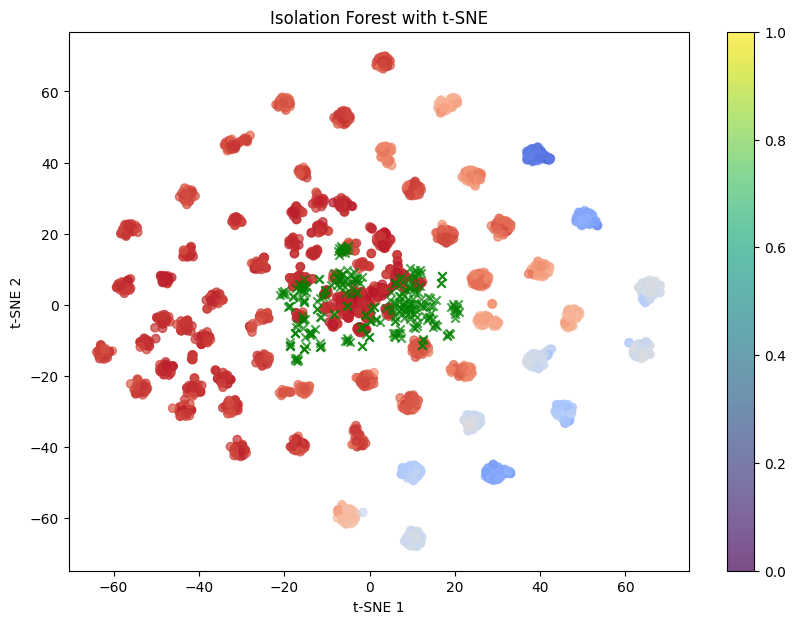
\includegraphics[width=\linewidth]{Graphics/isolation_forest_Tsne.png} % Nombre de la primera imagen
    %\caption{Primera imagen}
  \end{minipage}
  \hspace{0.5cm} % Espacio horizontal entre las dos imágenes
  \begin{minipage}[b]{0.45\linewidth}
    \centering
    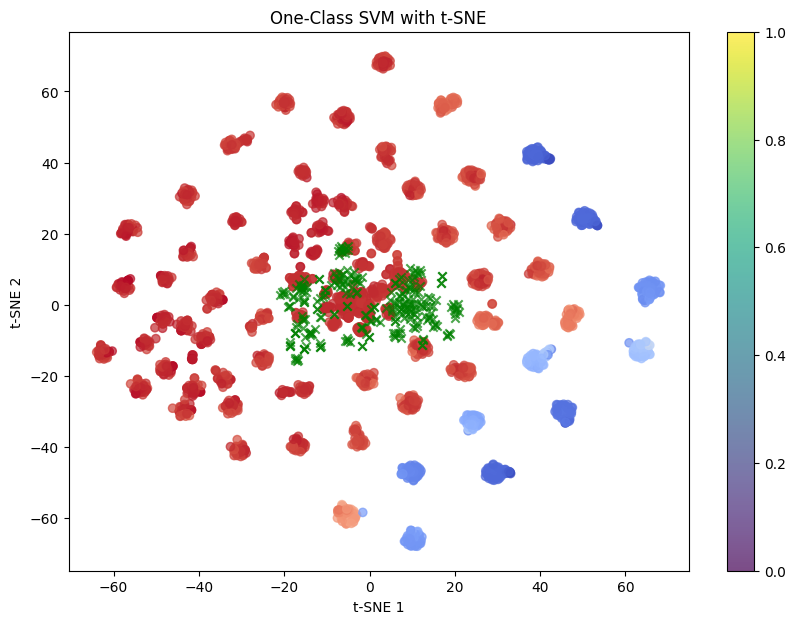
\includegraphics[width=\linewidth]{Graphics/one_class_svm_Tsne.png} % Nombre de la segunda imagen
    %\caption{Segunda imagen}
  \end{minipage}
\end{figure}


\begin{figure}[ht]
  \centering
  \begin{minipage}[b]{0.45\linewidth}
    \centering
    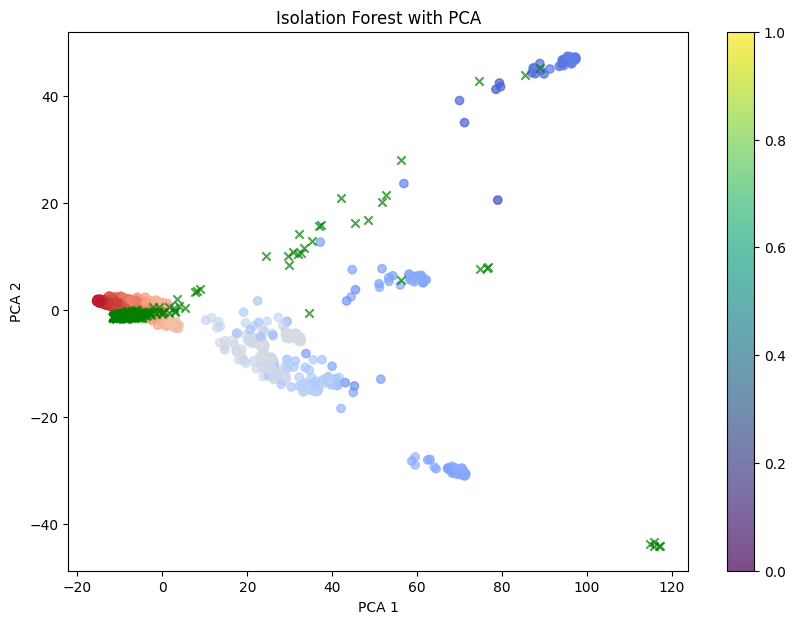
\includegraphics[width=\linewidth]{Graphics/isolation_forest_PCA.png} % Nombre de la primera imagen
    %\caption{Primera imagen}
  \end{minipage}
  \hspace{0.5cm} % Espacio horizontal entre las dos imágenes
  \begin{minipage}[b]{0.45\linewidth}
    \centering
    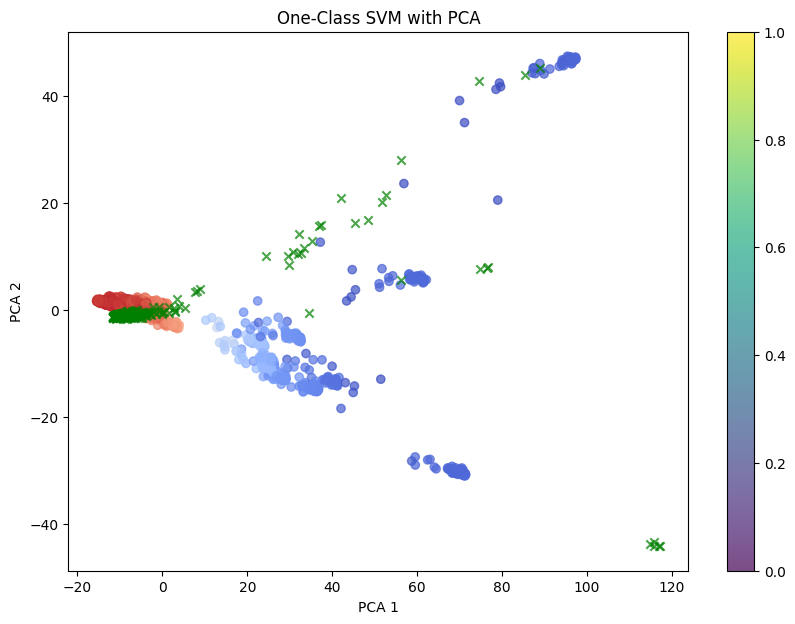
\includegraphics[width=\linewidth]{Graphics/one_class_svm_PCA.png} % Nombre de la segunda imagen
    %\caption{Segunda imagen}
  \end{minipage}
\end{figure}


\begin{table}[ht]
\centering
\begin{tabular}{lcc}
\toprule
\textbf{Modelo} & \textbf{Error en entrenamiento} & \textbf{Error en prueba} \\
\midrule
Isolation Forest & 388/3880 & 74/712 \\
One-Class SVM & 758/3880 & 147/712 \\
\bottomrule
\end{tabular}
\caption{Errores de Isolation Forest y One-Class SVM}
\label{tab:resultados}
\end{table}

Los resultados indican que tanto Isolation Forest como One-Class SVM muestran promesa en la identificación de anomalías dentro del espacio de vectores de similitud de código. Isolation Forest logró tasas de error más bajas en comparación con One-Class SVM en ambos conjuntos de entrenamiento y prueba, lo que sugiere que puede ser más efectivo para aislar muestras de código disímiles. Sin embargo, estos hallazgos son preliminares debido a problemas continuos con la extracción precisa del árbol de sintaxis abstracta. Por lo tanto, estas tasas de error aún no representan completamente el rendimiento final de los modelos.\\

Es importante destacar que las tasas de error reportadas están influenciadas por la calidad de la extracción del AST. ASTs inexactos o incompletos pueden llevar a una representación errónea de las estructuras de código, afectando así la evaluación del rendimiento de los algoritmos de detección de anomalías. Abordar estos problemas es crucial para obtener resultados más confiables.

\backmatter

\begin{conclusions}
    Conclusiones
\end{conclusions}

\begin{recomendations}
    Recomendaciones
\end{recomendations}

\printbibliography[heading=bibintoc]


\end{document}